\chapter{确定性数据核心：八阶段流水线（Dataset Core）}\label{ch:dataset-core}

Dataset Core 是系统唯一的数据信任边界。它将数据处理固定为八个阶段：采集、解析、规范化、兼容性检查、整合、多表组装、校验、发布。每个阶段都有明确的输入、输出摘要和执行凭证，记录该阶段产生了哪些文件及各文件的摘要。本章按阶段说明各环节对数据质量的实际作用。

\begin{figure}[htbp]
\centering
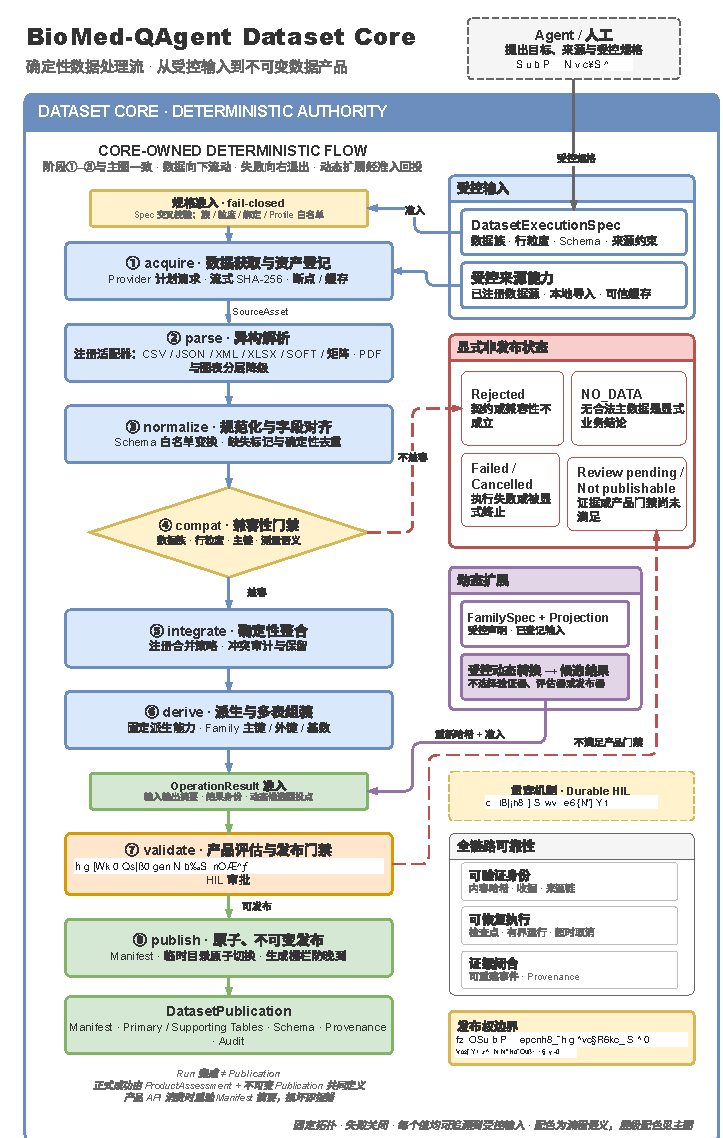
\includegraphics[width=0.66\textwidth]{figures/biomed-qagent-core-deterministic-flow.pdf}
\caption{Dataset Core 数据流。候选文件先接受检查，再进入正式发布；审批按请求类型执行。}\label{fig:core-deterministic-flow}
\end{figure}

Core 采用固定处理顺序，但输入与变换方案可以变化。静态路线使用已注册的数据家族；动态路线允许 Agent 提出多表结构和变换代码，先产生候选文件，再交给 Core 检查。变换方不能自行选择验证器、评估器或发布器。这里分开的是候选与正式文件，并不声称具备操作系统级沙箱隔离。

准入检查核对输入来源、输出表头和摘要是否与声明一致。例如输出列与声明不符时，系统返回 OUTPUT\_HEADER\_MISMATCH。通过这些检查仍可能存在计算或字段含义错误；这类问题需要审查变换方法并核对原始记录。开发记录也曾出现占位符文件通过旧检查的情况，因此不能从检查全部通过推导出数据必然正确。

Rejected、NO\_DATA、Failed 与 Cancelled 表示不同的非成功结果；等待审核也不等于已经发布。只有满足发布条件，系统才创建正式发布物。

\section{阶段1：正式采集与来源资产登记（acquire）}

Agent 的来源发现拿到URL 后，正式路线不会直接信任工作区中的任意文件。Core 的统一下载设施按预定的请求定义执行网络访问，实施访问策略、大小与超时限制、重试、断点续传和内容缓存。文件写入任务专属目录后，来源资产注册表流式计算SHA-256，把任务、来源身份、内容摘要、媒体类型与采集实现身份绑定为一份输入证据，支持时还记录快照或修订号等版本信息。因此，“来源资产”不是一个本地路径，而是可复核的输入证据。

\section{阶段2：异构数据解析（parse）}

正式静态路线使用已注册的解析器，把来源特有的CSV、JSON、XML、XLSX、SOFT、矩阵或API 响应转换为数据批次，同时输出解析统计、被拒绝的记录和溯源定位信息。解析器的原则是失败而不猜测：遇到来源格式异常时，解析器应失败或将问题写入审计记录，而不是让模型猜测缺失字段。

表达数据的解析集中体现了行层级纪律。GEO 既可能提供基因级结果，也可能只提供探针级矩阵；系统不会在缺少可信注释时把探针当成基因，一行究竟代表一个探针还是一个基因由表结构显式声明。GDC 与Xena 的输入形态不同，但都必须转换到目标表达表结构后才可合并。

论文衍生的载体单独处理。PDF 表格解析保留页面与位置证据（页码、边界框、题注），无框线表格与跨页表头仍是启发式解析难点，这类解析结果需人工核对。图表走视觉模型通道（4.2.1 节）。

\subsection{图表与视觉模型}\label{subsec:chart-vlm}

图表工具优先调用 qwen3.8-flash 读取页面或嵌入图像；调用或解析失败后，尝试 PDF 表格解析，再失败则仅保留图表标题。视觉提取只转录图内明确印出的数值，不将曲线像素位置估算为精确原始值。没有数值标注时，Agent 应继续检索正文表格、补充材料、出版社 source data 或作者仓库；仅识别曲线和描述趋势不计作数值数据交付。格式正确但数值错误的回答不会自动触发降级，仍需与来源核对。

VLM、PDF 表格或标题抽取结果先形成带来源定位的图表证据，再由数据家族组装。每个数据点记录抽取模型、置信度及其依据；人工修正保留原值和修改记录。样例6发布了六张关联表与三件说明文件，但存在这些文件并不等于图表数值已经完整取得；该案例的交付比较见\ref{subsec:gold6-artifact-compare} 节。

图系列表记录轴名、单位、刻度和图例，并声明含义明确、含义不明或已经人工确认。规则检查声明与点数据是否矛盾：例如标为“精确”的点不能同时对应含义不明的轴。轴状态若从一开始就误报为明确，此类一致性检查无法发现错误。因此，本文将其称为图表证据一致性检查，不等同于独立识别全部坐标轴或图例解析错误。点级样例测试只能证明相应检查路径可以执行，本轮尚未报告端到端数值误差率。

\section{阶段3：含义规范化与缺失、重复处理（normalize）}

规范化器依据目标表结构完成类型转换、字段命名统一、实体标识表达和必要的值标准化。核心原则是：只有目标表结构和规范化配置明确授权的变化，才可以自动执行；规范化过程保留原始写法与规范值之间的血缘，便于任何一处转换被事后复核。

缺失与重复按类型分层处理：必填字段缺失时拒绝或阻断，可选字段缺失保留为空并计入完整性统计；完全重复按确定性键去重；主键重复且值一致时合并血缘、保留多来源。每类处理都保留对应证据，以便后续复核。

实体身份对齐同样采用确定性机制：化合物以InChI Key 精确匹配建立交叉映射表，匹配不上时显式标记为冲突而不强行合并；基因符号归一使用内置确定性映射表；探针到基因的映射依赖逐平台注释资产，未映射探针保留原命名空间，不静默丢弃。这些注释资产与来源文件同样按内容摘要登记，映射结果随发布件交付。

\section{阶段4–5：兼容性检查与多源整合（compat、integrate）}\label{sec:stage5-integrate}

解析与规范化产物进入整合前，兼容性检查核对各批次在数据家族、表结构、行层级、实体层级、单位、含义和尺度上是否可以合并，并据此生成确定性的合并域键：值的含义、尺度与单位，加上物种、特征命名空间、测量类型、规范化状态与参考版本等维度，任何一维不一致都不能进入同一合并域。未知单位或不受支持的数值尺度不会被自动修正；单位换算只在有注册转换公式时执行，公式限定为线性安全形式，没有注册规则时阻断或交人工选择，系统不会自动“猜”一个换算。

整合器按注册策略合并批次。主键相同且数值一致时，保留多来源记录；数值冲突时，记录冲突键、双方取值与保留结果，必要时停止发布。采用先到优先处理同键冲突时，重跑也需要固定来源处理顺序。这种取舍使结果可以核对，并不说明先到来源更可靠。研究者可以根据证据重新判断，修正后另行发布。

\section{阶段6：多表组装（derive）}\label{sec:stage6-derive}

对于需要关联多个实体的数据，组装阶段生成多表候选，检查主键、外键、基数和表角色。\footnote{主键标识一行；外键指向另一张表的主键；基数说明两表记录是一对一、一对多还是多对多；表角色说明某张表记录测量值、身份信息或其他内容。}

单表与多表由数据关系决定。一个观测层级可以使用单表；测量值、实验条件与化合物身份需要分别保存时，再拆成关联表。生物活性表 activities 通过外键关联 assays 与 compounds，并辅以靶点、来源和交叉映射表（图~\ref{fig:bioactivity-fk}）。发布清单声明连接键与关系，下游无需根据同名列猜测如何拼接。

\begin{figure}[htbp]
\centering
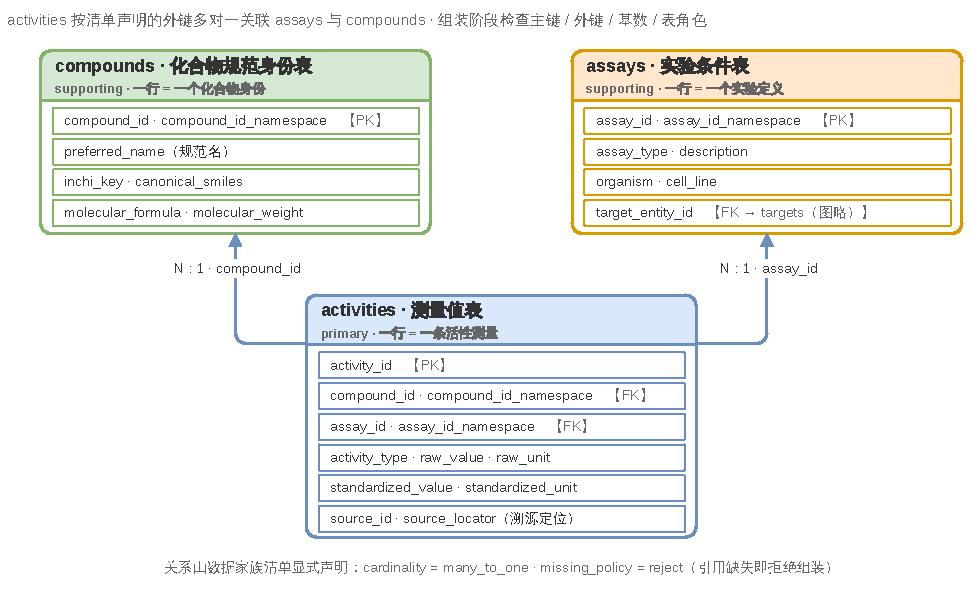
\includegraphics[width=0.94\textwidth]{figures/biomed-qagent-bioactivity-multitable-fk.pdf}
\caption{生物活性多表关系：activities 通过外键关联 assays 与 compounds。}\label{fig:bioactivity-fk}
\end{figure}

\section{阶段7：校验、置信度与产品评估（validate）}\label{sec:stage7-validate}

发布前检查字段类型、必填项与允许缺失率、主外键、实体命名空间、单位、来源定位、置信度记录，以及文件摘要和处理版本。多表产品评估从结构、关系、标识、溯源、置信度和复现所需信息六方面记录问题。没有阻断项时判为可发布；仍缺复现信息时，不能取得同等发布评级。这些规则检查文件是否符合声明，不能仅凭通过检查就认定科学含义全部正确。

置信度按证据类型分级。受版本约束的确定性解析可以取得 high；VLM、LLM、OCR 与网页抽取最高为 medium。该分级不是统计校准后的正确概率。本系统不会自动对全部 medium 记录发起人工审核；是否逐点复核与整个产品是否需要发布验收属于两项不同决定。未逐点复核的数值仍需对照原始来源，本轮没有测量各等级的实际错误率。

验证结论与明确的结束状态绑定。空主数据、兼容性失败或验证失败的结果一律不可发布；“运行完成”也不等于“发布物生成”。

\section{阶段8：不可变发布与消费时重验（publish）}\label{sec:stage8-publish}

发布器把质量检查合格的候选复制到独立目录，生成发布清单，逐文件记录相对路径、媒体类型、字节数和SHA-256；发布经临时目录原子切换完成，执行锁与代次围栏保证超时或已取消的旧执行不能晚到覆盖新结果。产品API 在每次读取时重新核验清单与文件摘要，文件被改动或损坏即拒绝展示。这里的“不可变”是应用层语义：正常API 只追加发布、不覆盖旧版本；系统不提供抵御同一操作系统账户重写文件系统的密码学防篡改能力。

\section{持久化人工确认与可恢复执行（Durable HIL）}\label{sec:hil}

字段映射不明确、单位未知、图表点置信度低或冲突无法按规则处理时，系统可以暂停并发出结构化请求。请求列出候选值、置信度、相关记录、证据摘要，以及任务、运行与需求身份。人工可以通过、拒绝或修正。恢复前必须核对请求是否仍有效、对象是否仍与审批证据一致；正常响应晚于请求发出时间，并不是拒绝恢复的理由。

请求分为工具许可、数据审核和发布验收。普通请求可按类型采用人工审核、模型初审或自动通过；模型初审不通过或调用失败时回退人工。对已经发起且属于强制人工类型的请求，非人工审批配置不被接受，只有人工处理后才继续。这个设置约束不单独证明每条动态发布路径都会触发验收：第五章样例7、样例9的归档运行没有业务 HIL 请求，因此本轮不能用它们证明动态发布一律经过人工确认。

\section{可靠性基座}\label{sec:reliability-base}

各阶段共用执行锁、取消检查、事件记录和文件重验。表~\ref{tab:reliability-base}区分设计约束与本轮可观察结果，避免将某次成功运行视为全部故障路径均已验证。

\begin{table}[htbp]
\centering
\caption{运行保护与检查依据}\label{tab:reliability-base}
\begin{tabularx}{\linewidth}{>{\hsize=0.60000\hsize}L>{\hsize=1.10000\hsize}L>{\hsize=1.30000\hsize}L}
\toprule
\textbf{措施} & \textbf{检查或控制的内容} & \textbf{依据与范围} \\
\midrule
执行锁 & 同一任务、同一需求不能并发写入同一发布目标 & 设计约束；并发行为需由专门测试检查 \\
代次围栏 & 发布前核对本次执行是否仍拥有写入权 & 用于阻止超时或取消后的旧执行继续发布 \\
超时与取消 & 操作有界；发布前检查取消状态 & 不能仅凭一次正常运行验证全部取消路径 \\
事件日志 & 追加操作与状态变化，供恢复与核对 & 本轮据事件起止时间和终态整理运行记录 \\
持久化人工确认 & 保存请求和决定，按原调用恢复 & 样例6记录了许可与发布验收；详见\ref{sec:hil} 节 \\
文件摘要与重验 & 读取时重算文件摘要，与清单比对 & 验证文件与回执一致，不验证重跑或科学正确性 \\
\bottomrule
\end{tabularx}
\end{table}

